\documentclass[a4paper]{article} 
\usepackage{amsmath}
\usepackage{amssymb}
\usepackage{graphicx}
%\usepackage[utf8]{inputenc}\
\usepackage[utf8x]{inputenc}
\usepackage{polski}
\usepackage[polish]{babel}
\usepackage[hidelinks]{hyperref}
\usepackage{color}
\usepackage{hyperref}
\usepackage{todonotes}
\usepackage{wrapfig}
\usepackage{float}
\usepackage[final]{pdfpages}
\usepackage{enumitem}
\usepackage{listings}
\usepackage{indentfirst}

\usepackage{chngcntr}
\counterwithout{section}{section}

%tikz
\usepackage{tikz}
\definecolor{blueish}{RGB}{33, 150, 243}
\definecolor{orangish}{RGB}{255, 152, 0}
\usetikzlibrary{arrows}
\tikzset{
  treenode/.style = {align=center, inner sep=0pt, text centered,
    font=\sffamily},
  arn_n/.style = {treenode, circle, white, fill=blueish,
    text width=1.5em},% arbre rouge noir, noeud noir
  arn_bn/.style = {treenode, rectangle, white, fill=blueish,
    inner sep=0.3em, minimum width=1em, scale=1, rounded corners=0.5em},% arbre rouge noir, noeud noir
  arn_l/.style = {treenode, circle, black, fill=orangish, text width=2.0em, very thick},% arbre rouge noir, noeud rouge
}

\hypersetup{
    colorlinks=false,
    linkcolor=blue,
    urlcolor=red,
    linktoc=all
}
\usepackage{geometry}
\lstset{basicstyle=\footnotesize\ttfamily}

\newcommand*\cpp{C\kern-0.2ex\raisebox{0.4ex}{\scalebox{0.8}{+\kern-0.4ex+}}}

\linespread{1.2}

\newtheorem{lemma}{Lemat}

\title{ORT}
\author{Adam Szady}

\begin{document}


{\let\newpage\relax\maketitle}

\begin{abstract}
Drzewa obszarów\footnote{(ang.) range tree} pozwalają zadawać zapytania o obszary ortogonalne w przestrzeni $n$-wymiarowej. Niniejszy dokument prezentuje ich strukturę, sposób tworzenia i przeszukiwania. Porównuje z alternatywnymi sposobami realizacji tego zagadnienia. Dostarcza też podstawową dokumentację programisty i użytkownika dla zaimplementowanej aplikacji.
\end{abstract}

\section{Cel pracy}
Projekt jest przedsięwzięciem realizowanym na potrzeby przedmiotu \emph{Geometria obliczeniowa}. Celem projektu było zaimplementowanie odpowiedniej struktury danych dla punktów na płaszczyźnie - drzewa obszarów, która pozwala szybko odpowiadać na zapytania o wszystkie punkty $q$ leżące w obszarze zadanym przez $x_1$, $x_2$, $y_1$, $y_2$. Ściślej rzecz ujmując, dla danego zbioru $P \subset \mathbb{R}^2$ wyznaczyć zbiór $Q$ taki, że $q \in Q \iff q \in P\ \land\ x_1 \le q_x \le x_2\ \land\ y_1 \le q_y \le y_2$.

Rozwiązanie powinno służyć jako narzędzie dydaktyczne do objaśnienia tworzenia struktury i realizacji zapytań.

\section{Teoria}
\subsection{Problem}
Praca uogólnia zadany problem. To ze względu na to, że nie sprawia większej trudności rozwiązanie powyższego zagadnienia dla dowolnej $n$-wymiarowej przestrzeni, ani uogólnienie go na dowolną funkcję $\boxplus$ (opisaną poniżej).

\subsubsection*{Ogólna definicja}
Dane są:
\begin{itemize}[noitemsep,topsep=0pt]
\item przestrzenie $X$, $V$, takie że $X \subseteq V$;
\item $n$ porządków liniowych $\prec_0$, $\prec_1$ ..., $\prec_{n-1}$ na $X$;
\item funkcja $\boxplus: V^2 \to V$ (łączna, przemienna\footnote{Przemienność nie jest wymagana w przypadku jednowymiarowym.});
\item (multi)zbiór $S \subset X$;
\item $A$, $B$ $\in X$.
\end{itemize}

Zadanie: znaleźć $p_1 \boxplus p_2 \boxplus p_3 \boxplus ...
 \boxplus p_k$, gdzie $p_1$, $p_2$, $p_3$, ..., $p_k$ to wszystkie punkty $p$ spełniające zależność $p \in S \ \land\ A \prec p \prec B$. Przy czym $x \prec y \iff x \prec_0 y \ \land\ x \prec_1 y \ \land\ ... \ \land\ x \prec_{n-1} y$.

\subsubsection*{Możliwe przypadki szczególne}
Łatwo zauważyć, że problem odnalezienia punktów dla obszaru ortogonalnego w przestrzeni dwuwymiarowej jest szczególnym przypadkiem tego problemu, dla:
\begin{itemize}[noitemsep,topsep=8pt]
\item $V = 2^{R^2}$, $X$ - zbiór singletonów $R^2$;
\item dwóch naturalnych porządków względem kolejnych współrzędnych;
\item $\boxplus(a, b) = a \cup b$;
\item $S$ - zbioru singletonów rozważanych punktów;
\item zaś $A = \{(x_1, y_1)\}$, $B = \{(x_2, y_2)\}$.
\end{itemize}

Przy użyciu tego mechanizmu można również rozwiązać chociażby problem znalezienia punktu o największej wadze. Wystarczy, że, mając zdefiniowaną dodatkowy porządek $\prec_w$, można przyjąć: $\boxplus(a, b) = \{a$ jeśli $b \prec_w a$, $b$ wpp. $\}$.

\subsection{Rozwiązanie - drzewa obszarów}
\subsubsection{Przypadek jednowymiarowy - $ORT_0$}
Wyobrażanie sobie $n$-wymiarowego rozwiązania najlepiej rozpocząć od rozwiązania jednowymiarowego.

Rysunek \ref{fig:tree1} przedstawia drzewo przedziałowe dla zestawu danych [2, 3, 5, 5, 5, 7, 8, 9]. Elementy są sortowane według zadanego porządku i umieszczane w liściach. Następnie drzewo tworzone jest w górę, by utworzyć pełne drzewo binarne. Do węzłów niebędących liśćmi przypisywana jest wartość funkcji $\boxplus$ dla dwóch synów. W ten sposób w dowolnym węźle tego drzewa mamy intuicyjnie rozumianą wartość funkcji $\boxplus$ dla całego poddrzewa - w tym przypadku sumy elementów.

\begin{figure}[!h]
\centering
\begin{tikzpicture}[->,>=stealth',
  level 1/.style={sibling distance = 4cm, level distance = .7cm},
  level 2/.style={sibling distance = 2cm, level distance = .85cm},
  level 3/.style={sibling distance = 1cm, level distance = 1cm},
] 
\node [arn_n] {44}
    child{ node [arn_n] {15} 
            child{ node [arn_n] {5} 
            	child{ node [arn_l] {2}}
							child{ node [arn_l] {3}}
            }
            child{ node [arn_n] {10}
							child{ node [arn_l] {5}}
							child{ node [arn_l] {5}}
            }                            
    }
    child{ node [arn_n] {29}
            child{ node [arn_n] {12} 
							child{ node [arn_l] {5}}
							child{ node [arn_l] {7}}
            }
            child{ node [arn_n] {17}
							child{ node [arn_l] {8}}
							child{ node [arn_l] {9}}
            }
		}
; 
\end{tikzpicture}
\caption{Jednowymiarowe drzewo przedziałowe z operacją dodawania}
\label{fig:tree1}
\end{figure}

\begin{lemma}
Przy założeniach, że zbiór $V$ ma skończoną moc\footnote{Ergo jego elementy mają złożoność pamięciową $\mathcal{O}(1)$},
zaś operacja $\boxplus(a, b)$ ma złożoność czasową $\mathcal{O}(|a|+|b|)$,
to dla $n = |S|$ w drzewie przedziałowym:
\begin{itemize}[itemsep=0pt]
\item Czas konstrukcji tego drzewa to $\mathcal{O}(n)$\footnote{Zakładając, że elementy te otrzymujemy w postaci posortowanej},
\item zajętość pamięci -- $\mathcal{O}(n)$,
\item zapytanie o przedział odbywa się w czasie $\mathcal{O}(\log{} n)$.
\end{itemize}
\end{lemma}

Nazwijmy tę strukturę $ORT_0$.

Co jednak, jeśli chcielibyśmy ograniczyć rozmiar elementów w węzłach przez rozmiar poddrzewa? Taka sytuacja następuje dla definicji $\boxplus(a, b) = a \cup b$.

\begin{lemma}
\label{lem:generalcplx}
Zakładając, że wielkość elementu drzewa, którego poddrzewo ma $m$ liści jest $\mathcal{O}(m f(m))$,
zaś operacja $\boxplus(a, b)$ ma złożoność czasową $\mathcal{O}(|a| f(|a|))$,
to dla $n = |S|$ w dziele przedziałowym:
\begin{itemize}[itemsep=0pt]
\item Czas konstrukcji tego drzewa to $\mathcal{O}(n f(n) \log{}n)$,
\item zajętość pamięci -- $\mathcal{O}(n f(n) \log{}n)$.
\end{itemize}
\end{lemma}

Zatem dla przypadku $\boxplus(a, b) = a \cup b$ mamy $f(m)=1$, zatem złożoność czasowa i pamięciowa konstrukcji takiego drzewa to $\mathcal{O}(n \log{} n)$. Oczywiście, w praktycznych zastosowaniach konstrukcja jednowymiarowego drzewa przedziałowego, obsługującego teoriomnogościową sumę jest straszliwym marnowaniem zasobów.

\subsubsection{Przypadek dwuwymiarowy - $ORT_1$}

Mając narzędzie do rozwiązania problemu w przestrzeni jednowymiarowej, rozważmy dodanie drugiego wymiaru (porządku).

Strukturę obsługującą dwa wymiary nazwiemy $ORT_1$, zaś jej elementami będą drzewa jednowymiarowe - $ORT_0$. Konstrukcję tego drzewa rozpoczynamy jak w przypadku $ORT_0$, zatem od posortowania elementów i umieszczenia ich w liściach.

Drzewo $ORT_1$ ma jednak w specjalny sposób zdefiniowaną funkcję $\boxplus$, która polega na utworzenia drzewa $ORT_0$ z wszystkich elementów danego poddrzewa. Funkcja ta będzie wykorzystywana jedynie podczas konstrukcji. Te drzewa niższego rzędu będą korzystały z innego porządku niż względem którego tworzone było $ORT_1$.

\begin{figure}[!h]
\centering
\begin{tikzpicture}[->,>=stealth',
  level 1/.style={sibling distance = 4cm, level distance = .7cm},
  level 2/.style={sibling distance = 2cm, level distance = .85cm},
  level 3/.style={sibling distance = 1cm, level distance = 1cm},
] 
\node [arn_bn] {$_0[8C,7E,2J,5G,5S,5Q,9V,3Y]$}
    child{ node [arn_bn] {$_0[2J,5S,5Q,3Y]$} 
            child{ node [arn_bn] {$_0[2J,3Y]$} 
            	child{ node [arn_l] {2J}}
							child{ node [arn_l] {3Y}}
            }
            child{ node [arn_bn] {$_0[5S,5Q]$}
							child{ node [arn_l] {5S}}
							child{ node [arn_l] {5Q}}
            }                            
    }
    child{ node [arn_bn] {$_0[8C,7E,5G,9V]$}
            child{ node [arn_bn] {$_0[7E,5G]$} 
							child{ node [arn_l] {5G}}
							child{ node [arn_l] {7E}}
            }
            child{ node [arn_bn] {$_0[8C,9V]$}
							child{ node [arn_l] {8C}}
							child{ node [arn_l] {9V}}
            }
		}
; 
\end{tikzpicture}
\caption{Dwuwymiarowe drzewo przedziałowe. $_0[x_1, ..., x_n]$ oznacza drzewo $ORT_0$ zbudowane z elementami $x_1, ..., x_n$. Zdefiniowane są dwa porządki na elementach - jeden względem cyfr, drugi względem liter.}
\label{fig:tree2}
\end{figure}

Korzystając z lematu \ref{lem:generalcplx} i zakładając, że czas konstrukcji i złożoność pamięciowa drzewa $ORT_0$ jest $\mathcal{O}(n \log{}n)$, otrzymujemy czas konstrukcji i złożoność pamięciową drzewa $ORT_1$ klasy $\mathcal{O}(n \log^2{}n)$.

\subsubsection{Przypadek $d$-wymiarowy - $ORT_{d-1}$}

Powyższe rozumowanie można łatwo uogólnić do dowolnej wymiarowości drzewa. Drzewo $ORT_{d-1}$ dla $d > 1$ będzie miało elementy w postaci drzew $ORT_{d-2}$. Stosując rozumowanie indukcyjne łatwo na podstawie lematu \ref{lem:generalcplx} wykazać, że złożoność czasowa i pamięciowa konstrukcji drzewa $ORD_{d-1}$ wynosi $\mathcal{O}(n \log^d{} n)$ jeśli drzewo $ORT_0$ było klasy $\mathcal{O}(n \log{} n)$.

Jeśli jednak założyć, że $\boxplus$ jest $\mathcal{O}(1)$, to otrzymujemy złożoności dla $ORT_0$ -- $\mathcal{O}(n)$, a~w~konsekwencji dla $ORT_{d-1}$ -- $\mathcal{O}(n \log^{d-1}{} n)$.

Pozostaje jedynie kwestia rozstrzygnięcia, w jaki sposób odpowiadać na zapytania. W drzewie najwyższego rzędu odnajdujemy wszystkie przedziały bazowe odpowiadające żądanemu zakresowi. Ich liczba w każdym wymiarze jest ograniczona przez $\mathcal{O}(\log{} n)$, zaś koszt ich odnalezienia to także $\mathcal{O}(\log{} n)$. Następnie, rekurencyjnie dla każdego z tych przedziałów bazowych, odpytujemy odpowiadające im drzewa niższego rzędu. Ostatecznie, ta rekurencyjna procedura zakończy się po $\mathcal{O}(\log{}^d n)$ krokach. W tym momencie już wystarczy tylko obliczyć funkcję $\boxplus$ na $\mathcal{O}(\log{}^d n)$ elementach. Ostateczna złożoność zapytania zależy zatem od jej charakteru. Dla zapytań o punkt o~największej wadze otrzymamy $\mathcal{O}(\log{}^d n)$, zaś dla zapytań o wszystkie punkty w obszarze mamy $\mathcal{O}(\log{}^d n + k)$, gdzie $k$ jest rozmiarem wyniku.

\section{Aplikacja}
Rozwiązanie zostało utworzone w języku \cpp 11. Dostarcza ono implementację ORT oraz przykładowe użycie.
\subsection{Testy wydajnościowe}
\label{sec:testy}

\begin{figure}[H]
\centering
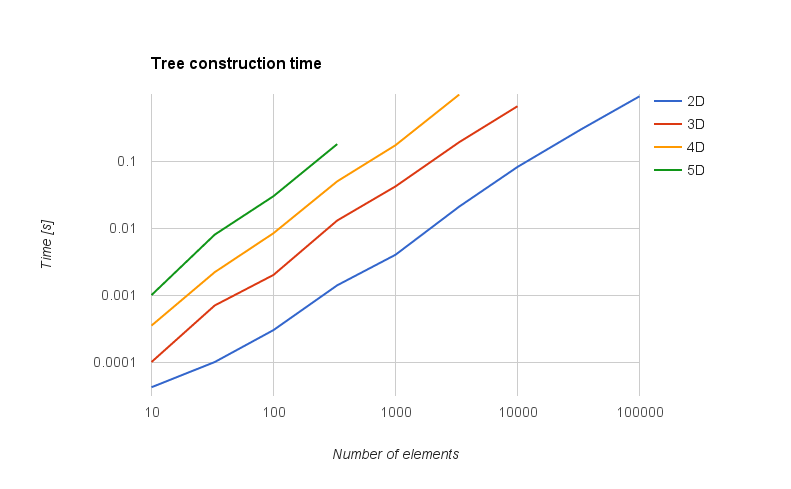
\includegraphics[scale=0.4]{Images/constr.png}
\caption{Czasy konstrukcji ORT}\label{fig:constr}
\end{figure}

\begin{figure}[H]
\centering
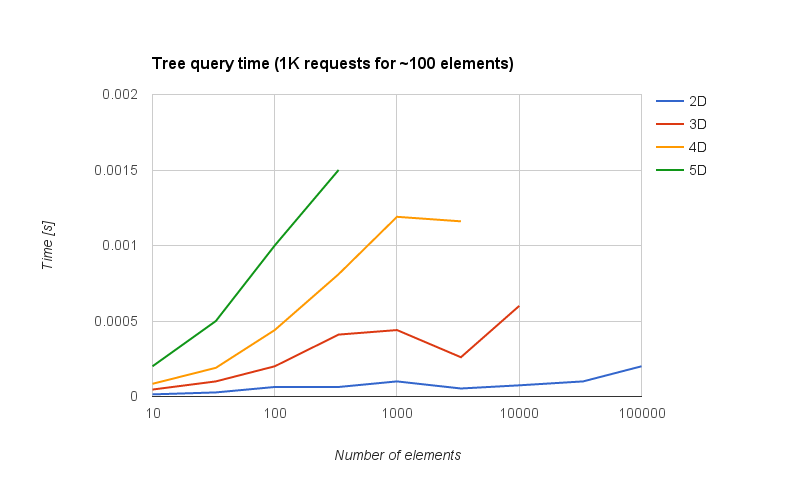
\includegraphics[scale=0.4]{Images/query.png}
\caption{Czasy zapytań ORT}\label{fig:query}
\end{figure}

Rysunki \ref{fig:constr} i \ref{fig:query} przedstawiają odpowiednio czasy tworzenia drzewa ORT i wykonywania zapytań - w zależności od liczby elementów oraz wymiarów. Założono rozkład równomierny we wszystkich wymiarach, w zakresie $[0;1)$. Zapytania o 100 elementów ograniczane były przez hipersześcian o boku $\sqrt[d]{100/N}$. Wykresy zdają się potwierdzać wyznaczone wcześniej teoretyczne złożoności obliczeniowe.

\subsection{Dokumentacja programisty}
Rozwiązanie dostarcza programiście klasę ORT.

Poniższy listing pokazuje przykładowy sposób konstrukcji drzewa dla przestrzeni 3D, w której punktom przypisano dodatkowy atrybut, względem którego będziemy chcieli odnajdywać maksimum.

\lstinputlisting[language=C++]{example.cpp}

W powyższym kodzie:
\begin{itemize}[noitemsep]
\item \textbf{NDPoint\textless Dim\textgreater } reprezentuje \emph{Dim}-wymiarowy punkt
\item \textbf{DimCmpSingle\textless Dim\textgreater ::precedes\textless IthDim\textgreater} -- \emph{IthDim}-ty porządek w \emph{Dim}-wymiarowej przestrzeni.
\item \textbf{MaxFn\textless Dim\textgreater} -- funkcję $\boxplus$
\item \textbf{ORT\textless Dim, V, DimCmp\textgreater(initial, mix)} -- konstruuje ORT o liczbie wymiarów \emph{Dim}, zbiorze $V=$\emph{V}, porządkach \emph{DimCmp} na danych \emph{initial}, wraz z funktorem \emph{mix} jako $\boxplus$.
\end{itemize}
\subsection{Dokumentacja użytkownika}

Dostarczona aplikacja demonstruje działanie struktury ORT w sposób dwojaki. Po pierwsze -- demonstruje wyszukiwanie punktów w obszarze ortogonalnym na płaszczyźnie (por. rysunek \ref{fig:viz}). Po drugie -- testuje wydajność struktur względem liczby wymiarów i~liczności zbioru punktów (opisanych w~\ref{sec:testy} \nameref{sec:testy}).

W pierwszej kolejności należy pobrać bibliotekę \emph{gogui} niezbędną do wizualizacji działania algorytmów. Przykładowo, może być to:
\begin{lstlisting}[language=bash]
  $ git clone https://bitbucket.org/mizmuda/gogui.git
  $ cd gogui
\end{lstlisting}

Następnie należy pobrać właściwą aplikację:
\begin{lstlisting}[language=bash]
  $ git clone https://github.com/aszady/ort.git
  $ cd ort
\end{lstlisting}

Oraz skompilować rozwiązanie przy użyciu \emph{cmake}:
\begin{lstlisting}[language=bash]
  $ cmake .
  $ make
\end{lstlisting}

Następnie aplikację można uruchomić poprzez polecenie:
\begin{lstlisting}[language=bash]
  $ ./ort
\end{lstlisting}

Po uruchomieniu aplikacja wypisze na standardowe wyjście wynik testów wydajnościowych, zaś do pliku \texttt{demoj.json} zapisany zostanie wynik wyszukiwania punktów na płaszczyźnie. Plik ten można przekazać do wizualizatora dostarczonego przez bibliotekę \emph{gogui} -- na przykład \texttt{gogui\_ vizualization/index.html} uruchomionego w przeglądarce z dostępem do odczytu plików lokalnych.

\begin{figure}[H]
\centering
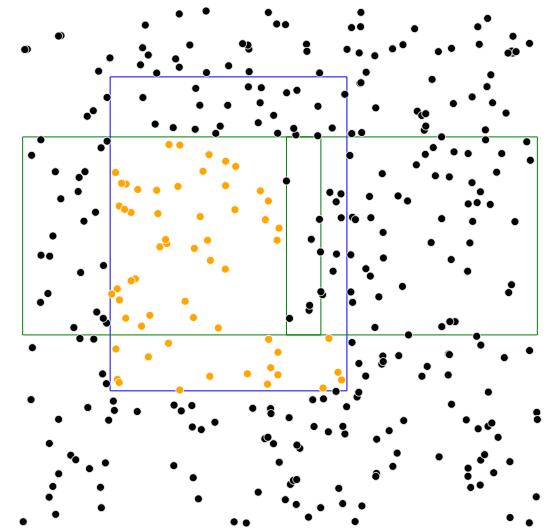
\includegraphics[scale=0.4]{Images/viz.png}
\caption{Fragment wizualizacji poszukiwania punktów na płaszcyźnie}\label{fig:viz}
\end{figure}

\section{Materiały}
\subsection*{Literatura}
\begin{enumerate}[noitemsep]
\item De Berg, Mark, et al. ,,Computational geometry.'' Computational geometry. Springer Berlin Heidelberg, 2000. 5.3-5.4.
\end{enumerate}
\subsection*{Odnośniki}
\begin{itemize}[noitemsep]
\item Prezentacja: \url{goo.gl/uoXWdn}
\item Kod: \url{github.com/aszady/ort}
\item Ten dokument: \url{https://github.com/aszady/ort/tree/master/doc/main.pdf}
\end{itemize}

\end{document}
